
% \begingroup
% \hyphenpenalty=10000
% \exhyphenpenalty=10000
% \begin{tikzpicture}[x=1cm,y=1cm,>=stealth]
% \path[use as bounding box] (0.15,0.20) rectangle (16.35,20.35);

% % Original colours preserved exactly.
% \definecolor{seqtext}{HTML}{1E293B}
% \definecolor{seqborder}{HTML}{475569}
% \definecolor{seqarrow}{HTML}{64748B}
% \definecolor{seqfill}{HTML}{DBEAFE}

% \tikzset{
%   seqparticipant/.style={rectangle,rounded corners=2.5pt,
%     draw=seqborder,fill=seqfill,line width=0.75pt,
%     minimum width=3.50cm,minimum height=1.80cm,text width=3.10cm,
%     align=center,text=seqtext,inner xsep=3pt,inner ysep=3pt,
%     outer sep=0pt,font=\sffamily\bfseries\fontsize{9.3}{11.2}\selectfont},
%   seqlifeline/.style={draw=seqarrow,dash pattern=on 3pt off 1.8pt,line width=0.72pt},
%   seqmessage/.style={->,draw=seqarrow,line width=0.80pt},
%   seqreturn/.style={seqmessage,dashed,line width=0.75pt},
%   seqactivation/.style={draw=seqborder,fill=seqfill,line width=0.65pt},
%   seqmessagetext/.style={text=seqtext,align=center,fill=none,
%     inner sep=2pt,outer sep=0pt,
%     font=\sffamily\fontsize{9.0}{10.8}\selectfont},
%   seqselftext/.style={seqmessagetext,anchor=west,align=left,
%     text width=2.80cm,font=\sffamily\fontsize{8.6}{10.3}\selectfont},
%   seqguard/.style={anchor=north west,text=seqtext,align=left,
%     text width=3.40cm,fill=none,inner sep=2pt,outer sep=0pt,
%     font=\sffamily\fontsize{8.4}{10.0}\selectfont}
% }

% % Equal participant widths, heights and horizontal spacing.
% \def\SeqIntentX{2.05}
% \def\SeqVerifyX{6.10}
% \def\SeqGraphX{10.15}
% \def\SeqControllerX{14.20}

% \node[seqparticipant] (intent) at (\SeqIntentX,19.30)
%   {Intent\\Validation};
% \node[seqparticipant] (verifier) at (\SeqVerifyX,19.30)
%   {Relationship\\Verification \&\\Decision};
% \node[seqparticipant] (knowledge) at (\SeqGraphX,19.30)
%   {Authoritative\\Verification Knowledge\\
%    {\mdseries\fontsize{8.4}{10}\selectfont Property Graph}};
% \node[seqparticipant] (controller) at (\SeqControllerX,19.30)
%   {Request\\Controller};

% % Lifelines start at the bottom of the participant boxes.
% \draw[seqlifeline] (intent.south) -- (\SeqIntentX,1.65);
% \draw[seqlifeline] (verifier.south) -- (\SeqVerifyX,1.65);
% \draw[seqlifeline] (knowledge.south) -- (\SeqGraphX,1.65);
% \draw[seqlifeline] (controller.south) -- (\SeqControllerX,1.65);

% % =========================================================
% % 1. Receive the validated intent
% % =========================================================
% \draw[seqactivation] ({\SeqIntentX-0.09},17.75)
%   rectangle ({\SeqIntentX+0.09},17.20);
% \draw[seqactivation] ({\SeqVerifyX-0.10},17.55)
%   rectangle ({\SeqVerifyX+0.10},11.65);
% \draw[seqmessage] ({\SeqIntentX+0.09},17.55) --
%   node[seqmessagetext,pos=0.5,above=4pt,text width=3.45cm]
%     {Validated Intent}
%   ({\SeqVerifyX-0.10},17.55);

% % =========================================================
% % 2. Determine the action-specific relationship pattern
% % =========================================================
% \draw[seqmessage] ({\SeqVerifyX+0.10},16.65)
%   -- (6.93,16.65) -- (6.93,16.05)
%   -- ({\SeqVerifyX+0.10},16.05);
% \node[seqselftext] at (7.13,16.35)
%   {Determine required\\relationship pattern};

% % =========================================================
% % 3. Request required relationships from the property graph
% % =========================================================
% \draw[seqactivation] ({\SeqGraphX-0.10},14.85)
%   rectangle ({\SeqGraphX+0.10},13.35);
% \draw[seqmessage] ({\SeqVerifyX+0.10},14.85) --
%   node[seqmessagetext,pos=0.5,above=4pt,text width=3.45cm]
%     {Resolve required\\relationships}
%   ({\SeqGraphX-0.10},14.85);

% % =========================================================
% % 4. Return evidence or a knowledge-access failure status
% % =========================================================
% \draw[seqreturn] ({\SeqGraphX-0.10},13.55) --
%   node[seqmessagetext,pos=0.5,above=4pt,text width=3.45cm]
%     {Verification Evidence /\\Failure Status}
%   ({\SeqVerifyX+0.10},13.55);

% % =========================================================
% % 5. Evaluate the relationships and validity of the evidence
% % =========================================================
% \draw[seqmessage] ({\SeqVerifyX+0.10},12.75)
%   -- (6.93,12.75) -- (6.93,12.15)
%   -- ({\SeqVerifyX+0.10},12.15);
% \node[seqselftext] at (7.13,12.45)
%   {Check relationships\\and evidence validity};

% % =========================================================
% % UML alt fragment: three distinct verification outcomes
% % =========================================================
% \draw[draw=seqborder,line width=0.75pt]
%   (5.30,1.65) rectangle (15.85,11.10);

% % Fragment operator tab.
% \fill[seqfill] (5.30,10.65) rectangle (6.18,11.10);
% \draw[draw=seqborder,line width=0.75pt]
%   (5.30,11.10) -- (6.18,11.10) -- (6.18,10.65) -- (5.30,10.65);
% \node[text=seqtext,font=\sffamily\bfseries\fontsize{9}{10.8}\selectfont]
%   at (5.74,10.875) {alt};

% % ---------------------------------------------------------
% % APPROVE
% % ---------------------------------------------------------
% \node[seqguard] at (6.47,10.40)
%   {[All mandatory relationships established;
%     evidence sufficient, current and valid]};
% \draw[seqactivation] ({\SeqVerifyX-0.10},9.00)
%   rectangle ({\SeqVerifyX+0.10},8.30);
% \node[seqactivation,rectangle,minimum width=0.26cm,
%   minimum height=0.68cm,inner sep=0pt,outer sep=0pt]
%   (approveReceiver) at (\SeqControllerX,8.65) {};
% \draw[seqmessage] ({\SeqVerifyX+0.10},8.65) --
%   node[seqmessagetext,pos=0.755,above=5pt,text width=3.38cm]
%     {\textbf{APPROVE}\\Approved Structured Verification Result}
%   (approveReceiver.west);

% \draw[draw=seqarrow,dashed,line width=0.65pt]
%   (5.30,7.70) -- (15.85,7.70);

% % ---------------------------------------------------------
% % REJECT: adequate knowledge supports a negative conclusion
% % ---------------------------------------------------------
% \node[seqguard] at (6.47,7.35)
%   {[Valid evidence and complete, current knowledge;
%     required relationships not established]};
% \draw[seqactivation] ({\SeqVerifyX-0.10},5.90)
%   rectangle ({\SeqVerifyX+0.10},5.20);
% \node[seqactivation,rectangle,minimum width=0.26cm,
%   minimum height=0.68cm,inner sep=0pt,outer sep=0pt]
%   (rejectReceiver) at (\SeqControllerX,5.55) {};
% \draw[seqmessage] ({\SeqVerifyX+0.10},5.55) --
%   node[seqmessagetext,pos=0.755,above=5pt,text width=3.38cm]
%     {\textbf{REJECT}\\Reason and Verification Evidence}
%   (rejectReceiver.west);

% \draw[draw=seqarrow,dashed,line width=0.65pt]
%   (5.30,4.85) -- (15.85,4.85);

% % ---------------------------------------------------------
% % Verification failure: no supported approval or rejection
% % ---------------------------------------------------------
% \node[seqguard] at (6.47,4.50)
%   {[Otherwise: evidence insufficient or invalid]};
% \draw[seqactivation] ({\SeqVerifyX-0.10},3.20)
%   rectangle ({\SeqVerifyX+0.10},2.50);
% \node[seqactivation,rectangle,minimum width=0.26cm,
%   minimum height=0.68cm,inner sep=0pt,outer sep=0pt]
%   (failureReceiver) at (\SeqControllerX,2.85) {};
% \draw[seqmessage] ({\SeqVerifyX+0.10},2.85) --
%   node[seqmessagetext,pos=0.755,above=5pt,text width=3.38cm]
%     {\textbf{Verification Failure}\\Reason / Failure Status}
%   (failureReceiver.west);

% \node[text=seqtext,align=center,
%   font=\sffamily\fontsize{8.3}{10}\selectfont] at (8.25,0.75)
%   {Begins after intent validation. Blockchain execution is outside this sequence.};
% \end{tikzpicture}
% \endgroup

\begingroup
\definecolor{seqtext}{HTML}{1E293B}
\definecolor{seqborder}{HTML}{475569}
\definecolor{seqarrow}{HTML}{64748B}
\definecolor{seqfill}{HTML}{DBEAFE}
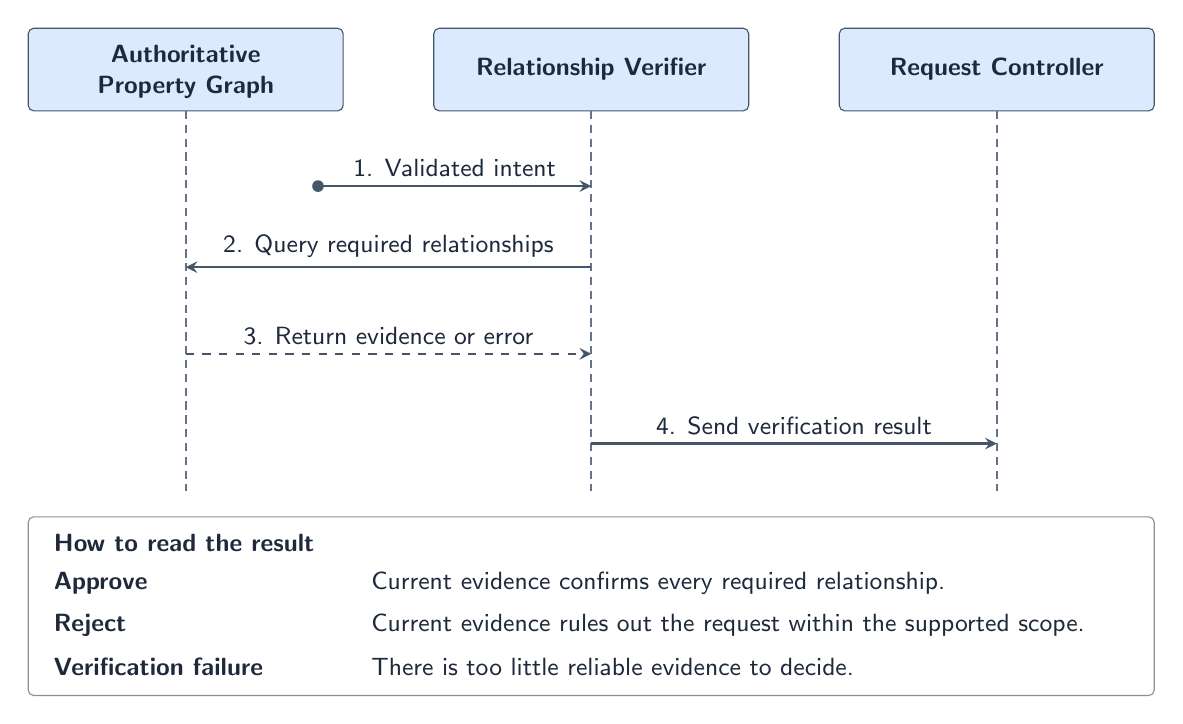
\begin{tikzpicture}[x=1cm,y=1cm,>=stealth,
 every node/.style={font=\sffamily\small,text=seqtext,align=center},
 head/.style={draw=seqborder,fill=seqfill,rounded corners=2pt,
   minimum width=4cm,minimum height=1.05cm,outer sep=0pt,
   font=\sffamily\bfseries\small},
 life/.style={draw=seqarrow,dash pattern=on 3pt off 2pt,line width=.6pt},
 msg/.style={->,draw=seqborder,line width=.85pt},
 lab/.style={above=2pt,inner sep=1pt},
 key/.style={anchor=west,align=left,inner sep=0pt}]
\node[head] (g) at (2.1,8.0) {Authoritative\strut\\Property Graph};
\node[head] (v) at (7.25,8.0) {Relationship Verifier};
\node[head] (c) at (12.4,8.0) {Request Controller};
\foreach \p in {g,v,c}
  \draw[life] (\p.south) -- (\p.south |- 0,2.65);

% All message tips terminate exactly on the recipient's lifeline.
\fill[seqborder] (3.78,6.52) circle (2.1pt);
\draw[msg] (3.78,6.52) -- node[lab]{1. Validated intent} (v |- 0,6.52);
\draw[msg] (v |- 0,5.49) -- node[lab]{2. Query required relationships} (g |- 0,5.49);
\draw[msg,dashed] (g |- 0,4.39) -- node[lab]{3. Return evidence or error} (v |- 0,4.39);
\draw[msg] (v |- 0,3.25) -- node[lab]{4. Send verification result} (c |- 0,3.25);

\draw[draw=seqborder!65,rounded corners=2pt] (.10,.05) rectangle (14.40,2.32);
\node[key,font=\sffamily\bfseries\small] at (.42,1.99) {How to read the result};
\node[key] at (.42,1.47) {\textbf{Approve}};
\node[key] at (4.45,1.47) {Current evidence confirms every required relationship.};
\node[key] at (.42,.94) {\textbf{Reject}};
\node[key] at (4.45,.94) {Current evidence rules out the request within the supported scope.};
\node[key] at (.42,.41) {\textbf{Verification failure}};
\node[key] at (4.45,.41) {There is too little reliable evidence to decide.};
\end{tikzpicture}
\endgroup